\documentclass[border=10pt]{standalone}
\usepackage{pgfplots}
\usepackage{tikz}
\pgfplotsset{width=13cm,compat=1.8}

\begin{document}
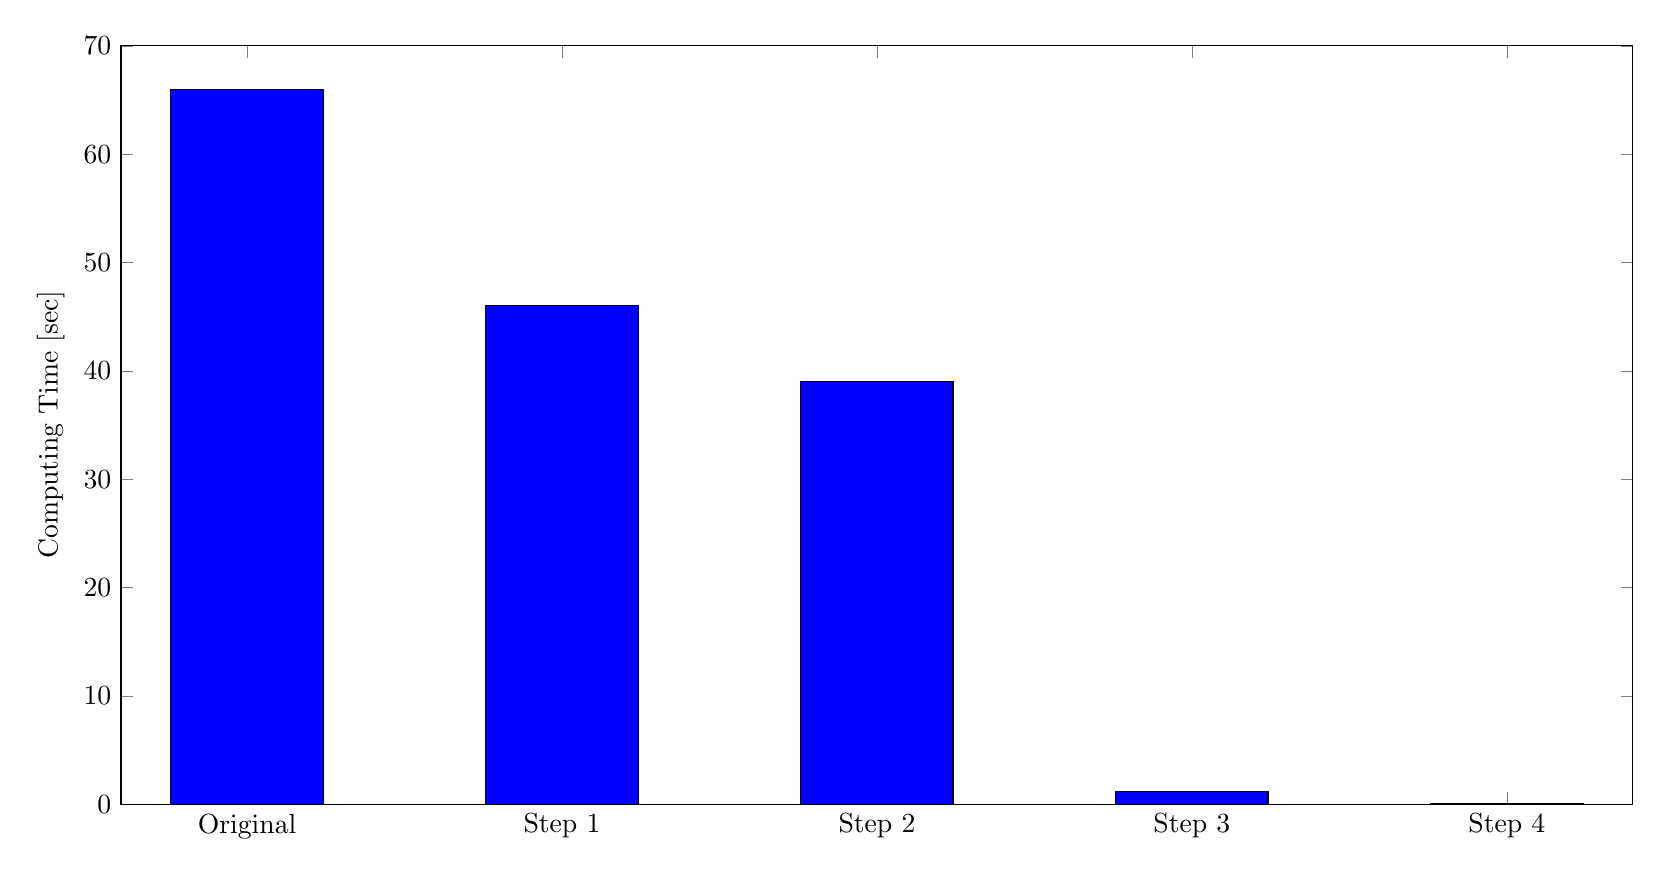
\begin{tikzpicture}[]
  \begin{axis}[scale=1.0,
	  ymax = 70,
	  ymin = 0,
      bar width=55pt,
      x=4cm,
      ylabel={Computing Time [sec]},
      symbolic x coords={Original,Step 1, Step 2, Step 3, Step 4},
      xtick={Original,Step 1, Step 2, Step 3, Step 4}
    ]
    \addplot[fill=blue,ybar] plot coordinates {
	    (Original, 66.0)
    };
    \addplot[fill=blue,ybar] plot coordinates {
	    (Step 1, 46.0)
    };
    \addplot[fill=blue,ybar] plot coordinates {
	    (Step 2, 39.0)
    };
    \addplot[fill=blue,ybar] plot coordinates {
	    (Step 3, 1.2)
    };
    \addplot[fill=blue,ybar] plot coordinates {
	    (Step 4, 0.1)
    };

  \end{axis}
\end{tikzpicture}

\end{document}
